%\setcounter{chapter}{2}

%    https://tex.stackexchange.com/questions/40725/how-to-change-the-font-size-during-the-new-defined-environment
%    http://www.sascha-frank.com/latex-font-size.html
%\begin{normalsize}
\begin{small}
%\begin{footnotesize}


\chapter{Physics Object Reconstruction}
\label{ch:cms_reco}

Excellent spatial resolution of the CMS trackers, high granularity of the calorimeters, and almost $4\pi$ coverage of the detector, allowed the CMS to introduce the particle flow (PF) algorithm \cite{Particle_flow} for a global event reconstruction. PF takes the input from all subdetectors, analyses the redundant information, removes the duplicate one, and forms the physics objects. PF procedure starts with identification of tracks and calorimeter clusters, then the reconstruction of the physics objects is performed, such as electrons, muons, jets, etc. In this section we will discuss the whole PF approach and all key elements of this reconstruction sequence.
  
  
\section{Track Reconstruction}\label{sec:track_reconstruction}

The reconstruction starts with the clusters of signals (``hits'') in the inner tracker. The information from these clusters in the Pixel and Strip subdetectors is aggregated based on their signal-to-noise ratios. The charge-weighted averaging is performed (for different particle charge hypothesis), as well as other corrections are further applied to identify the real hit positions. 

The helix trajectory that the particle follows in the magnetic field inside of the detector is characterised by five parameters: the direction in $\eta$, the 3D position with respect to the reference point, which is the centre of the IP, and the curvature of the track with the radius R. This information is enough to compute estimates of basic physics quantities, however, the this task is complicated by the presence of event high multiplicity (number of charged particles produced in the same event) and also by the physics aspect of the electron propagation in matter: an electron traversing the detector has nearly 85 $\%$ probability to emit a bremsstrahlung photon. Hadronic effects also need to be taken into account: a hadron has a 20 $\%$ probability to experience multiple scattering on the nuclei of the detector before reaching the HCAL. 

To keep the track finding efficiency high, while maintaining low the efficiency of miss-identified tracks, track reconstruction is performed sequentially using the combinatorial track finder (CTF) \cite{combined_track_finding}. First the "purest" tracks are reconstructed, they have high $p_T$ and the hits point towards the primary vertex (PV). The term PV is used to refer to the vertex which is the actual point of origin of the produced particle, when several other hard scattering vertices are present in the event. Then these pure tracks are removed from the collection of tracks and another round of the track reconstruction starts. This procedure applied several times reduces the combinatorial factor and also simplifies the identification of tracks with the low $p_T$ or those which do not point to the PV. During each iteration, the reconstruction follows these steps:

\begin{itemize}
\item Seed generation. Rough estimates of the particle trajectories ("seeds") are produced using either three hits or two hits and a PV constraint. Based on which iteration the algorithm is at, some additional constraints are applied, e.g., a minimal $p_T$ requirement, the need for the seed to originate close to the beam spot, etc. 
\item Trajectory building. Initial seeds are projected towards the compatible hits in the next layers based on the Kalman Filter (KF) procedure \cite{Kalman_filter}. The extrapolation is done until the outermost layer of the tracker is reached or when a "terminating condition" is satisfied, e.g., when the iteration accumulated the maximum number of invalid hits ("fake hits"). Each obtained trajectory is updated using a KF approach based on the compatibility of hits to form a better track candidate. The procedure is complicated by the fact that the same initial seed can give rise to several track candidates or vice versa, the same track candidate may be compatible with different seeds. Additionally, the trajectory building step should take into account energy loses of the particle due to multiple scattering on the detector material, inhomogeneities of the tracker material, and the effects of the regions of non constant magnetic field. 
\item Track fitting. After the track candidate has been built, the track parameters are refitted by a KF and the "smoother". This step uses the full available information about the track and gives optimal estimates of the track parameters. To remove a large number of fake tracks, which are present due to a very complicated nature of the problem and the high track multiplicity in the event, a multivariate (MVA) selection is applied. MVA incorporates variables that discriminate real tracks from the fakes: the signed transverse curvature and impact parameters (with respect to the beam spot), the polar and azimuthal angles, number of missing hits, the fit quality variables, etc. 
\end{itemize}

The CTF procedure runs for 10 iterations. For 2016 collisions with a mean pileup (additional hard scattering vertices) of 24, the CTF efficiency to identify real tracks varied from 80 to 95$\%$ with the mis-identification efficiency of 5 - 10 $\%$.



\subsection{Muon tracking}\label{sec:muon_track_reconstruction}

Muons are detected by the inner tracker and also by the outer (muon) tracker. This greatly improves muon track reconstruction and motivated the development of a dedicated muon reconstruction algorithms. The ninth and the tenth iterations of the CTF are focused on the muon reconstruction. These iterations are using three separate algorithms to identify: 

\begin{itemize}

\item Standalone muons. This algorithms uses only muon tracker information: DTs, CSCs, RPCs. Hits from the inner chambers are used as seeds and projected to hits in the outer chambers. Then, a standard KF procedure is used to identify track candidates, which are called standalone muons.
\item Tracker muons. Only the inner tracking information is used to form tracks. Tracks are further projected to muon subsystems, where a compatibility with at least one muon hit is required. This algorithm works with low momentum muons: tracks with $p_T$ above 0.5 GeV and a total momentum greater than 2.5 GeV.
\item Global muons. Tracker tracks and standalone tracks are projected to the outermost layer of the muon system, checking the compatibility between two approaches. The resulting combined set of track hits is refitted to produce a global muon track. Mostly high momentum muons with $p_T > $ ?? 200 GeV profit from this algorithm.
\end{itemize}


\subsection{Electron tracking}\label{sec:ele_track_reconstruction}
Electrons are also detected by the inner tracker, however, their reconstruction is complicated by the fact that they emit bremsstrahlung photons and the trajectory becomes more complex. As a result, the clustering algorithms need also to identify the bremsstrahlung photons and account for the fact that the energy clusters corresponding to these photons may be located outside of the main electron trajectory, when extrapolated to the ECAL. 

Since a KF approach assumes that energy losses are Gaussian, and this is not the case for electrons, a dedicated procedure is developed - a modified KF - the Gaussian Sum Filter (GSF) \cite{GSF}. In this method the radiated energy losses are approximated by the sum of Gaussian distributions. 

The electron seeds for the GSF are built using the ECAL information. Two different approaches are developed for the track reconstruction:

\begin{itemize}

\item Super Cluster based electrons. Cluster of energy in the ECAL and grouped together to form super clusters (SCs). Using the information of the energy spread among the clusters, the curvature of the electrons is estimated and tracker seeds are formed, with the SC position as a constraint. 
\item Tracks based electrons. Tracks from the inner tracker are projected to ECAL clusters, checking the compatibility using quality variables, such as $\chi^2$, number of missing hits (absent hits along the path of the track), etc. 
\end{itemize}

A typical momentum resolution for electrons in $Z \rightarrow e^- e^+$ decays is approximately 1.7 - 4.5$\%$.

\subsection{Primary Vertex reconstruction}\label{sec:PV_reconstruction}

At the LHC energies, several hard scattering vertices are produced in each collision. The location of all primary vertices (PV) is reconstructed using the tracks. However, normally only one (the main PV) out of these vertices (referred to as additional vertices or pileup) produces the interesting physics interactions. All the vertices are important since they are reused in the feed-back loop of the track reconstruction procedure. Also, a precise identification of primary vertices is important for determining the effect of the pileup on all physics objects in general and b-tagging in particular (will be discussed later in this chapter). 



The PV identification consists of three steps: the tracks are selected, then the tracks from the same PV are combined in clusters, and, finally, the position of the PV is determined from the fits to tracks.

Selecting the tracks, only those consistent with the location of the PV are considered. Several variables are used to improve the quality of the track selection procedure: the transverse impact parameter (the relative distance in the vertical plane with respect to the centre of the beam spot),  the number of strip and pixel hits associated with a track, and the $\chi^2$ of the fit .

Clustering of the tracks is based on their z position with respect to the beam spot. A deterministic annealing (DA) algorithm \cite{DeterministicAnnealing} is used to find the global minimum for this problem with many degrees of freedom. The idea of this algorithm is based on the physics example of a system approaching a state of minimal energy through a series of temperature  reductions. 

Once the clustering is completed and PVs are identified, the candidates with more than two tracks are fitted using an adaptive vertex fitter \cite{AdaptiveVertexFitting}. The result of this procedure is a set of probabilities assigned to tracks. This can be thought of as a likelihood that the track originated from the given vertex.


The resolution of PVs varies between 10 - 100 $\mu$m to 100 ?m and depends on track qualities. The main PV is determined as the vertex with the highest sum of the squared $p_T$.


\subsection{Particle Flow links and blocks}\label{sec:some_reconstruction}

Usually a particle leaves the signal in several CMS dubdetectors which is stored as PF \cite{ParticleFlow} elements. To connect these PF elements, the link algorithm (LA) was developed. The LA can test any pair of elements in the event. To speed up the calculations, only pairs of elements that are "neighbours" in the specified $\eta - \varphi$ plane are considered. When the pair of elements is linked, the LA determines the distance between the elements which is related to the quality of the link. This procedure produces PF blocks of elements, which are connected either by a direct or an indirect link (through the common elements)

The procedure produces inner tracker-calorimeter, HCAL-ECAL cluster-to-cluster, ECAl-ECAL, and ECAL-Preshower links. In most cases the link distance is defined as the $\eta-\varphi$ or $x-y$ distance between the two cluster positions. In case of the ambiguity when, e.g., several HCAL clusters are linked to the same ECAL cluster, only one link is kept - with the smallest distance. 

The last stage of the link algorithm is dedicated to formation the inner tracker-muon system links. Once all links are established and PF blocks are formed, the PF algorithm proceeds reconstructing objects in the following sequence: muon candidates (with corresponding PF tracks and clusters been removed from the PF block), electron candidates (taking into account bremsstrahlung photons) and high momentum isolated photons (with related tracks and clusters also been removed), and, finally, charged hadrons and non-isolated photons.

The elements that are still left in the PF blocks are then re-considered for another round of identification of: charged hadrons and neutral hadrons, photons from parton fragmentation and hadronization, and jet decays. Lastly, when all PF blocks have been sorted out, the global event description is completed and the reconstructed event is re-processed by a post-processing step (PP step), which addresses the possible particle misidentification and misreconstruction during the previous steps. 




\subsection{Muons}\label{sec:muons}

Muon reconstruction is the first stage of the PF algorithm. It identifies muons using global and inner tracker muon properties. Global muon candidates are selected at this step and the isolation requirement (explained later in this chapter) is applied. 
This isolation requirement is efficient enough to reject hadrons mis-identified as muons. 

The muons inside jets or secondary muons from hadron decays are complicating the identification of prompt muons, such as those originating from Higgs, W, or Z boson decays. Therefore, additional more stringent selection is further applied. 


For non-isolated global muons, in addition to the Tight WP selection, it is required to have more than two matching track segments in the muon detectors or that the calorimeter energy deposits are compatible with the muon candidate. This selection discriminates against the high $p_T$ hadrons. 

If muons fail Tight WP, there are still several "recovery" iterative procedures that use the relax the selection criteria. 

However, even at this stage the muon identification and reconstruction is not finished. Charged hadrons reconstructed during the next PF stages can be reconsidered as muon candidates. Only after the whole PF sequence is completed, including the PP step, the PF algorithm terminates.


%%%%%%%%%%%%%%%%%%%%%%%%%%%%%%%%%%%%
 
All muons considered for this measurement are global muons that satisfy the Tight WP requirements (Tight WP as an initial selection) with extra requirements on the number of hits in the tracker and muon system, on the impact parameter, and the quality of the global track. 

The efficiency $\epsilon$ to successfully identify a prompt isolated lepton (in our case muon or electron) can be decomposed as:

$\epsilon = \epsilon_{tracker} \cdot \epsilon_{ID | tracker} \cdot \epsilon_{ISO | ID} $

\noindent where the first term refers to the tracker efficiency, the next term is the Bayesian term which refers to the identification (ID) efficiency given that the lepton already passed the tracker requirements, and the final term refers to the isolation (ISO) efficiency given that the lepton already satisfied identification criteria. All the efficiencies are well optimised in the CMS and are in the range from 85 to more than 99 $\%$ depending on the $p_T$ and $\eta$ of the lepton (muon in this case). 

The muon resolution for 20 to 100 GeV momentum range varies from 1 $\%$ in barrel to 5 $\%$ in endcaps.

\subsection{Electrons and isolated photons}\label{sec:electrons}

The reconstruction of electrons is complicated by the fact that they lose energy emitting bremsstrahlung photons and, thus, their trajectory becomes more complex than the one of muons. Additionally, bremsstrahlung photons often convert to $e^+ e^-$ pairs. And this is a recursive process: daughter electrons also emit photons. Due to this complication, the procedure to reconstruct electrons and photons is similar. First a GSF track plays a role of the seed for the electron candidate. An ECAL SC with no links to the GSF track is used as a seed for the photon candidate. For both electron and photon candidates energy deposits in the HCAL must not exceed 10$\%$ of the ECAL energy. 


Then all ECAL clusters in the PF block are linked to the SC or to one of the GSF track tangents of the candidate. The total energy of the collected ECAL clusters is corrected for the energy losses during the linking procedure and is assigned to photons. 
The electron candidate is formed from a combination of the corrected ECAL energy and the electron direction given by the GSF track. Additional MVA discriminator of O(20) variables is applied to improve electron identification efficiency. The MVA approach based on the Boosted Decision Trees (BDT) classifier \cite{TMVA} profits from the following highly discriminating variables: the amount of energy radiated off the GSF track, the distances between the ECAL SC position and the projection from the GSF track, track-cluster linking variables, KF and GSF track quality variables, etc. 


Photon candidates are kept if photons are isolated and the corresponding configuration of ECAL energy deposits is compatible with those expected from a given photon shower.  


All identified electron and photon tracks and clusters in the PF block are masked before the algorithm starts processing hadrons. 
Since some offline physics analyses may apply different selection for electrons and photons, PF selection is relatively loose and  the full electron and photon reconstruction information is saved in case a different re-interpretation must be run. This allows to save time in the future since would not require running the complete PF algorithm again.




\subsection{Hadrons and non-isolated photons}\label{sec:hadrons}

After the muons, electrons, and isolated photons get reconstructed, they are removed from the PF blocks. The next PF algorithm iterations proceed with hadrons from jet fragmentation and hadronization. These particles can be seen by the detector as charged pions, kaons or protons, neutral pions and kaons, and non-isolated photons from neutral pion decays. During the reconstruction, the precedence is given in the ECAL to photons over neutral hadrons. This priority does not hold above $|\eta| > 2.5$. In that region ECAL clusters linked to a given HCAL cluster are identified as hadrons and, only if ECAL clusters are without such a link, then they are classified as photons.  


What is left in the PF block, gets classified in the following manner: if energy deposits are consistent with the energy hypothesis from the tracker, then no neutral hadron is found and each track that remains - corresponds to a charged pion candidate. 

In situations when the energy deposits in the ECAL does not match well the energy hypothesis from the tracker and this discrepancy is larger than three standard deviations, a new muon reconstruction starts, with the relaxed muon selection. This approach allows to improve the muon identification efficiency without increasing the mis-identifiedmuon rate. 


If the track momentum sum is still significantly larger than the calorimetric energy,the excess in momentum is often found to arise from residual misreconstructed tracks with apTuncertainty in excess of 1 GeV. These tracks are sorted in decreasing order of theirpTuncer-tainty and are sequentially masked either until no such tracks remain in the PF block or until


The hadron traversing the material of the tracker interacts with the nuclei of the tracker and often produces secondary hadrons. These hadrons evidently are produced outside of the PV - at the secondary (intermediate) interaction  vertex. When the charged-particle tracks corresponding to these secondary particles are linked together, the resulting secondary particle candidates can be  replaced  in  the  list of reconstructed  particles by a single (original) charged hadron.  

Estimate of the energy of the primary charged hadron is then given by:

$E = E_{secondary} + f \cdot p_{primary}$

\noindent where $E_{secondary}$ is a vectorial sum of the momenta of the secondary charged particles, $p_{primary}$ is the momentum of the incoming track, and $f$ is the factor determined from the simulations. 


%%%%%%%%%%%%%%%%%%%%%%%%%%%%%%%%%%%%%%%%%

\subsection{Jets and jet corrections}\label{sec:jets}

Jets are collimated streams of particles created in the fragmentation and hadronization process of the original parton, quark or gluon. As jets propagate through the CMS detector, they leave tracks in the tracking system and interaction showers  in the calorimeter crystals. 


Several jet reconstruction algorithms have been developed. In the Higgs boson group of the CMS, most measurements are using $anti-k_T$ algorithm \cite{antiKt}. If the jet clustering uses PF particles - PF jets are reconstructed. If only the ECAL and HCAL information is used - calorimeter jets are identified ("calo jets"). When all stable particles (in case of the simulation, at the generator level) excluding neutrinos are used - reference jets are reconstructed ("Ref jets"). In this measurement PF $anti-k_T$ jets are used. 



The anti$-k_T$ algorithm is one of the cone algorithms that takes as input a collection of PF objects inside of the cone of the radius R (usually defined by the jet size). The algorithm defines the distance parameter:
$d_{ij} = \min (\frac{1}{p^2_{T_i}}, \frac{1}{p^2_{T_j}}) \times \frac{R^2_{ij}}{R}$,

\noindent where $p_{T_i}$ and $p_{T_j}$ refer to the transverse momenta of PF particles $i$ and $j$, $R_{ij}$ is the distance in the $\eta - \varphi$ plane. 


An additional $d_{iB}$ parameter is defined as the distance between the particle $i$ and the beam axis: $d_{iB} = \frac{1}{p^2_{Ti} }$.

The algorithm iteratively finds the minimum distance choosing at each step the minimal value in the ($d_{ij}$, $d_{iB}$) pair, using a collection of the PF particles as an input.  

If the minimum distance is $d_{ij}$, then the four-vectors of $i$ and $j$ particles are summed to form a new particle. Particles $i$ and $j$ are removed from the initial input collection. If the minimum distance is $d_{iB}$, then the particle $i$ is considered a jet. This particle is also removed from the set of particles and the algorithm continues until all initial particles have been combined into jets. The mechanics of the algorithm clusters soft candidates with the hardest particles first, producing a perfect cone-shaped jets.



PF jets are used in this thesis over Calo jets since the former have a superior angular resolution. PF algorithm allows the precise determination of the charged hadron direction and momentum, while in calorimeters, the energy deposits of charged hadrons are spread along the $\varphi$ direction in the presence of the magnetic field. This gives an extra degradation of the azimuthal angular resolution of jets.


On average, the jet energy is formed by: 65$\%$ by charged hadrons, 25$\%$ by photons, and 10$\%$ by neutral hadrons. The possibility to identify the contributors to the total jet energy during the jet reconstruction is one of the reasons to use the PF algorithm for jet reconstruction. In practice the identification of particles inside jets is done comparing the jet energy fractions measured in PF jets to those of the corresponding Ref jets.


To remove the jet energy dependence on p$_T$ and $\eta$ of the jet and, hence, to "flatten" the corresponding two dimensional map, the jet energy correction (JEC) procedure is introduced. Additionally, the jet energy resolution (JER) correction is necessary. The latter is defined as the Gaussian width of the ratio of the energies of the corrected PF jets to Ref jets. Both corrections improve the angular resolution, energy response, and energy resolution of jets. 


JEC scales the four-momentum of jets. The various detector effects are addressed. Depending on how sensitive the physics analysis is to this correction type, one can factorise this correction into separate components and apply them individually in a sequence. Most important individual corrections remove: energy contributions due to pileup, effects of the calorimeter response, residual Data-MC discrepancies, effects of the jet flavor, etc.

JER smears the four-momenta of reconstructed jets to match the energy resolution observed in data. The smearing procedure derives the correction factors which scale the reconstructed jet momentum with respect to the the same jet clustered from the generator MC level.


\subsection{The b tagging and secondary vertices}\label{sec:btag}

In this measurement one of the Higgs bosons decays to b quarks. Jets produced during the hadronisation of b quarks  are called b jets. A dedicated b tagging is necessary since Higgs boson decay to b quarks has the highest branching fraction of almost 58$\%$ and is a great test of the SM validity. 


B quarks will produce jets that contain B mesons, which have a relatively long lifetime $c \tau \approx 500 \mu$ m. This distance travelled at almost the light speed would correspond to a dislocation of a few mm from the PV. The new positions where the B meson decays, will be clearly seen in the detector. This displaced vertex, the secondary vertex (SV), is a unique signature of b quarks and is used to identify their decays. Sometimes the vertex cannot be unambiguously reconstructed, but even in these cases the properties of tracks within b jets are different from the ones originating from gluons or light quarks (light jets).



After passing the selection criteria, tracks are considered for b tagging. The selection requirements, that include kinematic and impact parameter properties of tracks, are needed to reject fake tracks, tracks coming from pileup vertices, and tracks from the long-lived hadrons. 


Two main approaches are used to reconstruct the secondary vertices (SV). One of the methods that pioneered the b tagging is an adaptive vertex reconstruction (AVR) algorithm. AVR is based on the adaptive vertex fitter, it uses the tracks associated with jets and finds PVs and SVs. The other algorithm is the inclusive vertex finder (IVF). IVF uses all the tracks in the event and is implemented with the selection looser than for the AVR. 

As for the b tagging itself \cite{CMS-PAS-BTV-15-001, Sirunyan:2017ezt}, multiple algorithms (taggers) have been developed and successfully used over the last decade. The most known ones are: 

\begin{itemize}

\item the jet probability (JP) and the jet b probability (JBP) tagger. Both are based on the probability of a jet candidate to be compatible with the PV using impact parameter significance (IPS) variables.
\item The soft electron tagger (SET) and soft muon tagger (SMT). These taggers are based on the presence of soft leptons within jets. It focuses on leptonic decays of B hadrons.
\item The combined secondary vertex (CSVv2) tagger. This is a more complex tagger based on the MVA technique. It uses displaced tracks and secondary vertices to tag b jets and takes as input IPS, decay length, SV parapeters, number of SVs, etc. This tagger can use both AVR and IVF vertices.
\end{itemize}

In this physics analysis a new MVA based (cMVAv2) tagger was used. This superior tagger uses the outputs from all the aforementioned "fundamental" taggers: JP and JBP, SET and SMT, CSVv2 using both AVR and IVF vertices. These ensemble learning procedure \cite{ensemble_learning}, that combines outputs from fundamental taggers into one complex MVA based tagger that produces the final output, is a popular machine learning technique that has been proven to lead to better results than the ones achieved by individual algorithms separately. 

\subsection{Missing transverse momentum}\label{sec:met}


When neutrinos are present in the event, they cannot be directly detected by the CMS, specific neutrino detectors would be needed in this case. However, using the CMS detector one can indirectly estimate the momentum of neutrinos. This procedure relies on the methods of the  missing  transverse  momentum \PTslash (or missing transverse energy  \ETslash (MET)). 

MET is constructed using all PF particles in the event and is calculated as:

$\PTslash = \vec{p}^{miss}_T = |- \sum^N_i \vec{p_{Ti}} |$. 

To reconstruct $\PTslash$, the CMS relies on almost $4 \pi$ coverage of the detector and precise measurement of the particle properties using PF algorithm that takes information from all subsystems. Produced $\PTslash$ is still considered "raw", since is not JEC and JES corrected. After these corrections are applied, one obtains  $\PTslash$ that is called "Type-1 corrected MET". This is the definition of MET that is recommended by the CMS JetMET particle Object Group (POG) group and is used in this measurement. Additional set of filters and corrections is further applied to reject events with artificially large $\PTslash$ due to the presence of several noise sources, such as ECAL dead cells, poor quantity muon candidates, HCAL noise. 




\subsection{Lepton isolation}\label{sec:isolation}

As mentioned before, lepton isolation is a great method to remove clear fakes and select real  prompt  muons  and  electrons  produced  by Higgs boson decay or by the weak decays of Z or W bosons. The isolation quantifies the activity of other particles around the particle of interest. The lepton isolation is defined as the scalar sum of the $p_T$'s of all charged and neutral hadrons and photons inside a cone of the radius $\Delta R <  0.3 - 0.4 $(depending on the working point (WP)). The sum is normalised by the $p_T$ of the lepton of interest:

$I_{PF} = \frac{1}{p_T} (\sum^\gamma p^\gamma_T + \sum^{h \pm} p^{h \pm}_T + \sum^{h^0} p^{h^0 }_T)$



\subsection{Pileup interactions}\label{sec:pileup}


Pileup interactions which have produced charged hadrons reconstructed as tracks can be identified as additional primary vertices (see Sec. 2.3.1). These hadrons can therefore be flagged as pileup and removed from the list of candidates in the event. This procedure is dubbed charged-hadron subtraction (CHS), and it should be understood that the reconstruction algorithms described in previous sections are based on CHS-cleaned candidate collections (PF+CHS) [188].
For neutral hadrons, photons, and charged hadrons beyond tracker acceptance or not
removed by CHS, no such straightforward procedure is possible. In one strategy pursued,
the average pT density due to pileup is estimated, relying on the uniformity of pileup
energy deposits. This density, ?, can then be multiplied by the ?area? A of a candidate,
and the result ? � A subtracted from the candidate?s pT. For jets, A is taken to be their
catchment area [203,204]. The effective area Aeff used to correct the electron isolation [194] 2
is directly related to the area of the isolation cone, (?R) , and their (absolute) isolation is then given by


PF
??
p +max?0, p + p ??A ?, (2.12.) T ? T T eff?
�?0i??? i?h i?h
??
e,abs. ??i ????i ??i ??
�0
where the sums run over all PF charged CHS (h ) and neutral (h , ?) candidates within
a cone of ?R ?? 0.3 around the electron. An alternative method, used to correct muon isolation, is based on the observed ratio of ?? ? 0.5 between neutral and charged pileup energy. The contribution to the isolation due to neutral pileup can therefore be estimated locally from the measured charged pileup energy in the isolation cone:
?,abs. ?? i ?? ?? i ?? i ?? i??
Iso ?? p +max?0, p + p ??? p ? (2.13.)
PF T ? T T T?
�?0i??�? i ? h i ? h i ? PU h
??
Here the sums run over the same collections as in (2.12), in a cone of ?R ?? 0.4 around the muon. In the last term of (2.13), only charged hadrons associated with pileup vertices are considered.
miss
The calibration of the pT is not expected to be affected by pileup, since pileup
miss
interactions produce little to no true pT . However, its resolution can be significantly
miss degraded due to the extra energy in the events. In addition to computing the p??T using
CHS-cleaned candidates, a correction for the effect of neutral energy deposits, referred to as Type-0 correction, is applied. This correction is computed from the observed charged pileup candidates, assuming that for pileup the true charged and neutral total transverse momenta are exactly balanced, and that the charged candidates are perfectly measured.





Pileup particles give rise to additional deposits in the calorimeters, approximately uniformly distributed throughout the detector, that degrade the energy
miss
resolution of jets and of the pT . Extra hits from charged pileup particles in the trackers
render track reconstruction more difficult due to the increased combinatorial background, resulting in a lower tracking efficiency and higher fake rate. As a consequence, but also due to the additional reconstructed tracks in the event, tasks such as b tagging become more challenging as well. Finally, the extra energy due to pileup impacts the estimate of lepton isolation, resulting in lower muon and electron selection efficiencies for a given isolation requirement. This sections describes the methods used to mitigate these effects

%%%%%%%%%%%%%%%%%%%%%%%%%%%%
  
  - somewhere a section on physics objects where you discuss that there are tracks, there are jets, there are b-jets, what it means an isolated lepton, what it means missing momentum, and so forth. For example, Ekaterina has a section on particle flow, if I remember right, where she discusses that. Or you can have a section that just discuses the proton-proton collisions environment and explains that many particles created in collisions are unstable and decay right away. What is observable in an experiment such as CMS is longer-lived or stable particles. These include electrons, muons, photons, and some ground state hadrons. At the same time, energetic quarks or gluons hadronize and can be seen in a particle detectors as jets of hadrons (so define jets here). Same for tau leptons, we detect them either as electrons/muons, or hadronic jets. Etc. If you have such a conceptual paragraph here, some time later you can have a particle flow discussion when it is time to be more specific. But discussion at this level above would allow you to then discuss the requirements on CMS design using terms like b-jets or isolated leptons.




\begin{figure}[H]
  \centering
  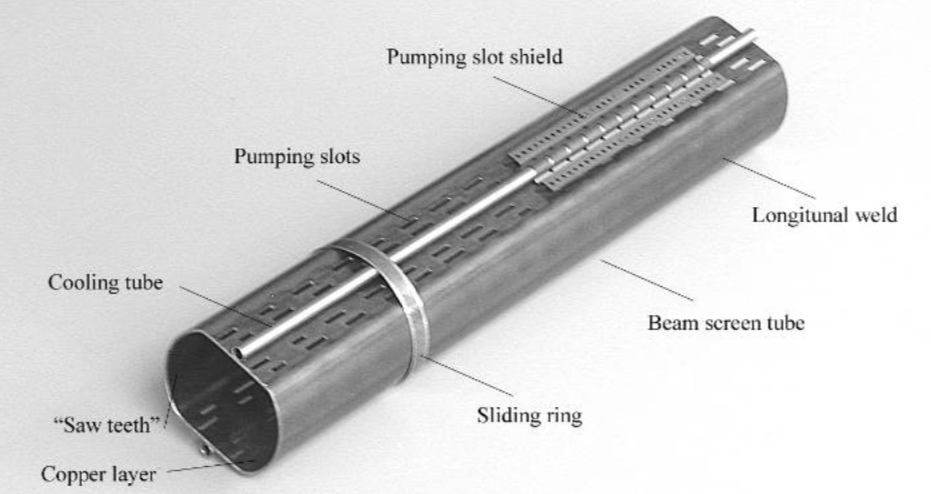
\includegraphics[width=0.7\textwidth]{beam_screen}
  \caption{Beam screen.}\label{beam_screen}
\end{figure}






  EGAMMA AT LEAST SAY THAT HAS BEEN WORKING AND SHOW SOME PLOTS?



%\end{normalsize}       % 28 to 58 -> 31 pages for the chapter (font 12)
\end{small}             % 28 to 56 -> 29 pages for the chapter (font almost 11)
%\end{footnotesize}  % 28 to 51 -> 24 pages for the chapter (font 10)
 
